\documentclass{article}
\usepackage{tikz}
\usetikzlibrary{shapes.multipart}
\newcommand\mathprobe[2]{%
  \setbox0=\hbox{$#2$}%
  \typeout{MATH #1: \the\wd0,\the\ht0,\the\dp0}%
}
\makeatletter
\newcommand\nodeprobe[2]{%
  \begin{tikzpicture}
    \node[#2] (probe) at (0,0) {$x$};
    \pgfpointanchor{probe}{center}%
    \typeout{NODE #1: center=\the\pgf@x,\the\pgf@y}%
    \pgfpointanchor{probe}{base}%
    \typeout{BASE #1: \the\pgf@x,\the\pgf@y}%
  \end{tikzpicture}%
}
\newcommand\anchorprobe[1]{%
  \pgfpointanchor{#1}{center}%
  \typeout{ANCHOR #1: \the\pgf@x,\the\pgf@y}%
}
\newcommand\partprobe[2]{%
  \pgfpointanchor{#1}{#2}%
  \typeout{PART #1/#2: \the\pgf@x,\the\pgf@y}%
}
\makeatother
\begin{document}
\mathprobe{x}{x}
\mathprobe{y}{y}
\mathprobe{r}{r}
\mathprobe{alpha}{\alpha}
\mathprobe{sin}{\sin x}
\mathprobe{sum}{x+y}
\mathprobe{cdot}{\cdot}
\mathprobe{pi}{\pi}
\mathprobe{equal}{x=y}
{\footnotesize\mathprobe{eight}{x}}
{\large\mathprobe{twelve}{x}}
{\small\mathprobe{small-log}{\log x}\mathprobe{small-ratio}{x/2}}
\nodeprobe{above}{above,thick}
\nodeprobe{south}{anchor=south,thick}
\nodeprobe{below}{below,line width=2pt}
\nodeprobe{north}{anchor=north,line width=2pt}
\nodeprobe{left}{left,outer sep=3pt}
\nodeprobe{east}{anchor=east,outer sep=3pt}
\nodeprobe{rotated-above}{above=2pt,rotate=30,inner xsep=5pt,inner ysep=1pt}
\nodeprobe{rotated-south}{anchor=south,yshift=2pt,rotate=30,inner xsep=5pt,inner ysep=1pt}
\nodeprobe{center-last}{above,anchor=center}
\nodeprobe{above-last}{anchor=center,above}
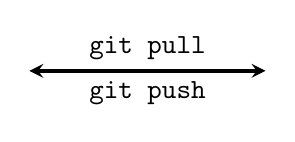
\begin{tikzpicture}
  \draw[very thick,stealth-stealth] (1.5,0)
    -- node[above] (pull) {\tt git pull} node[below] (push) {\tt git push} (4.5,0);
  \anchorprobe{pull}\anchorprobe{push}
\end{tikzpicture}
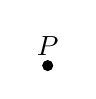
\begin{tikzpicture}
  \fill (0,0) circle (2pt) node[above] (p) {$P$};
  \anchorprobe{p}
\end{tikzpicture}
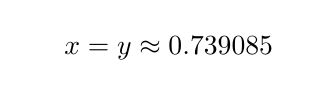
\begin{tikzpicture}
  \node[label={[name=angular,label distance=0.1cm]0:$x = y \approx 0.739085$}] at (1,1) {};
  \anchorprobe{angular}
\end{tikzpicture}
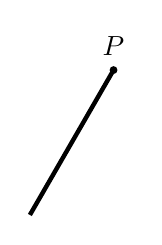
\begin{tikzpicture}[scale=0.85]
  \draw[ultra thick,rotate=60] (0,0) -- (2.5,0) coordinate (B);
  \draw[xshift=-1cm] (B) node[circle,fill,inner sep=1pt,label={[name=label]above:$P$}] (e) {};
  \anchorprobe{e}\anchorprobe{label}
\end{tikzpicture}
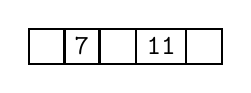
\begin{tikzpicture}[font=\tt,thick]
  \node[rectangle split,rectangle split horizontal,rectangle split parts=5,draw,
    rectangle split empty part width=1.5] (split)
    {\nodepart{one}\nodepart{two}7\nodepart{three}\nodepart{four}11\nodepart{five}};
  \partprobe{split}{north}\partprobe{split}{south}\partprobe{split}{two}\partprobe{split}{four}
\end{tikzpicture}
\end{document}
